% ===================
% OFFICIAL BAU THESIS FORMATTING SETTINGS - DO NOT MODIFY
% ===================
% WARNING: DO NOT MODIFY THE DOCUMENT CLASS, PACKAGES, OR SETTINGS BELOW
% These are the official BAU settings required for thesis formatting compliance
% Any changes to the preamble may result in formatting violations and
% rejection of your thesis submission
%
% Last Updated: September 2025
% Complies with: BAU Graduate Studies Requirements
%
% Prepared and maintained by the IT Department – Beirut Arab University
%
% Go to the \begin{document} line to start editing the document
% ===================



\documentclass[a4paper,12pt]{report}
\usepackage{geometry}
 \geometry{
 a4paper,
 top=2.5cm,
 bottom=2.5cm,
 left=3.18cm,
 right=2.5cm}
\renewcommand{\contentsname}{Table of Contents}
\usepackage[utf8]{inputenc}
\usepackage{indentfirst}
\usepackage{times}
\usepackage[shortlabels]{enumitem}
\usepackage[numbers,sort&compress]{natbib}
\usepackage{subcaption}
\usepackage{multirow}
\usepackage{adjustbox}
\usepackage{caption}
\usepackage{comment}
\usepackage[dvipsnames]{xcolor}
\usepackage{tocloft}
\usepackage{rotating}
\usepackage{lineno,hyperref}
\usepackage{xurl}
\usepackage{graphicx}
\usepackage{array}
\usepackage{pdfpages}
\usepackage{chngcntr}
\usepackage{pgfplots}
\pgfplotsset{compat=1.18}
\usepackage{tikz}
\usetikzlibrary{shapes.geometric, arrows.meta, positioning}

\tikzset{
  startstop/.style={
    circle, draw, minimum size=0.6cm, line width=1pt
  },
  process/.style={
    rectangle, draw, minimum width=5cm, minimum height=0.8cm,
    text centered, line width=1pt, font=\small
  },
  arrow/.style={
    -{Stealth[length=6pt]}, line width=1pt
  }
}
\usepackage[acronym]{glossaries}
% Use noidx so abbreviations work with pdflatex alone (no separate makeglossaries run).
\makenoidxglossaries

\bibliographystyle{unsrtnat}

\let\printorcid\relax % Remove ORCID footnote
\input{acronyms}

\hypersetup{
  colorlinks=false,
  pdfborder={0 0 0}
}

% Compile from \texttt{research/} with assets at repo root (e.g.\ \texttt{../University-Logo/}).
\graphicspath{ {figures/}{../} }

% Define list of equations
\newlistof{myequations}{loe}{List of Equations}
\newcommand{\listequationsname}{List of Equations}
\newcommand{\listofequation}{\listofmyequations} % Compatibility wrapper

% Format to match List of Figures style
\setlength{\cftmyequationsnumwidth}{2.3em}
\setlength{\cftmyequationsindent}{1.5em}
\newcommand{\myequation}[2][]{%
  \begin{equation}
    #2
    \ifx&#1&%
      \addcontentsline{loe}{myequations}{\protect\numberline{\theequation}#2}
    \else
      \addcontentsline{loe}{myequations}{\protect\numberline{\theequation}#1}
    \fi
  \end{equation}
}

% Alternative command for equations with labels
\newcommand{\myequationlabel}[3][]{%
  \begin{equation}\label{#3}
    #2
    \ifx&#1&%
      \addcontentsline{loe}{myequations}{\protect\numberline{\theequation}#2}
    \else
      \addcontentsline{loe}{myequations}{\protect\numberline{\theequation}#1}
    \fi
  \end{equation}
}

\linespread{1.5} 
\title{\textbf{TITLE} \\}
\author{AUTHOR \\}
\date{}

\counterwithout{equation}{chapter} 
\setcounter{secnumdepth}{3}
\setcounter{tocdepth}{3}
\usepgfplotslibrary{colormaps}

% =====================
% CUSTOMIZATION INSTRUCTIONS
% =====================
% Replace the following placeholders with your information:
% 1.  [THESIS TITLE] - Your complete thesis title
% 2.  [Student Full NAME] - Your full name
% 3.  [Master's/PhD] - Your degree type
% 4.  [PROGRAM TITLE] - Your program 
% 5.  [DEPARTMENT TITLE] - Your department 
% 6.  [FACULTY TITLE] - Your faculty 
% 7.  [YEAR] - Submission year
% 8.  [SUPERVISOR NAME] - Primary supervisor's name
% 9.  [POSITION AND TITLE] - Supervisor's academic position
% 10. [COMMITTEE MEMBERS] - Names of all committee members
% 
% Additional notes:
% - Add or remove sections as needed for your thesis
% - Optional sections can be removed if not applicable
% - Maintain consistent formatting throughout
% =====================


\begin{document}

\begin{titlepage}
\thispagestyle{empty}
\centering
\vspace*{1cm}

\includegraphics[width=0.5\textwidth]{University-Logo/logo.png}

\vspace{2cm}


{\fontsize{16}{20}\selectfont\textbf{ICT Competition Research Project Report}}

\vspace{1cm}

% Title
{\fontsize{16}{20}\selectfont\textbf{DDoS Attack Detection Using ResNeXt50-32x4d with MindSpore}}

\vspace{1cm}


{\fontsize{14}{18}\selectfont by}

\vspace{1cm}

% Student Full Names
{\fontsize{16}{20}\selectfont\textbf{Mohamad Al Ghoush - 202300735}} \\[0.2cm]
{\fontsize{16}{20}\selectfont\textbf{Abed Al Rida Nehme - 202303149}} \\[0.2cm]
{\fontsize{16}{20}\selectfont\textbf{Wafik Ibrahim - 202301238}} \\[0.2cm]
{\fontsize{16}{20}\selectfont\textbf{Ahmad Sharkawi - 202300122}}

\vspace{1cm}

% Department and Faculty
{\fontsize{12}{16}\selectfont
Electrical and Computer Engineering, Faculty of Engineering\\[0.3cm]
Computer Engineering Program
}

\vfill

% Year
{\fontsize{12}{16}\selectfont 2026}

\end{titlepage}

% Second Title Page - Same as first but with supervisors
\begin{titlepage}
\thispagestyle{empty}
\centering

% University Logo
\vspace*{1cm}
\includegraphics[width=0.5\textwidth]{University-Logo/logo.png}


\vspace{2cm}

{\fontsize{16}{20}\selectfont\textbf{ICT Competition Research Project Report}}

\vspace{1cm}

% Title
{\fontsize{16}{20}\selectfont\textbf{DDoS Attack Detection Using ResNeXt50-32x4d with MindSpore}}

\vspace{1cm}


{\fontsize{14}{18}\selectfont by}

\vspace{1cm}

% Student Full Names
{\fontsize{16}{20}\selectfont\textbf{Mohamad Al Ghoush - 202300735}} \\[0.2cm]
{\fontsize{16}{20}\selectfont\textbf{Abed Al Rida Nehme - 202303149}} \\[0.2cm]
{\fontsize{16}{20}\selectfont\textbf{Wafik Ibrahim - 202301238}} \\[0.2cm]
{\fontsize{16}{20}\selectfont\textbf{Ahmad Sharkawi - 202300122}}



% Department and Faculty
{\fontsize{12}{16}\selectfont
Electrical and Computer Engineering, Faculty of Engineering\\[0.3cm]
Computer Engineering Program
}

\vspace{1cm}

% Supervised by
{\fontsize{14}{18}\selectfont\textbf{Presented to}}

\vspace{1cm}

% Supervisors table

\begin{tabular}{c@{\hspace{0.5cm}}c@{\hspace{0.5cm}}c}
\textbf{Eng. Mustafa Bizri}
\end{tabular}

\vfill

% Year
{\fontsize{12}{16}\selectfont 2026}



\end{titlepage}


\indent
\pagenumbering{roman}
\newpage
\chapter*{Abstract}
\addcontentsline{toc}{chapter}{Abstract}
This report describes a deep learning system for detecting SYN flood
\gls{ddos} attacks from raw network traffic. Traffic is converted into grayscale
images under a \textbf{0.3\,s time-window} aggregation (primary model
\mbox{\texttt{per\_second\_0p3\_focal\_v2}}), trained and evaluated on splits from
\mbox{\texttt{images\_per\_second\_window\_0p3}} derived from the public CICDDoS2019
dataset. A ResNeXt-50 (32$\times$4d) \gls{cnn} in Huawei MindSpore with
\mbox{\texttt{mindcv}} performs binary classification (DDoS vs.\ benign), using focal
loss and DDoS-focused early stopping. Reported test accuracy is about
\textbf{98.1\%} with macro F1 \textbf{0.937} (offline same-domain evaluation,
2026-04-03). A companion live pipeline on CPU logs window-level predictions;
those lines are \textbf{not} calibrated to offline accuracy without labeled
capture in deployment.

\vspace{1em}
\noindent\textbf{Keywords:} SYN flood DDoS; packet-to-image encoding; ResNeXt; MindSpore; \mbox{CICDDoS2019}; intrusion detection.

\newpage
\tableofcontents
\newpage
\listoftables
\addcontentsline{toc}{chapter}{List of Tables}
\newpage
\listoffigures
\addcontentsline{toc}{chapter}{List of Figures}
\newpage
\listofequation
\addcontentsline{toc}{chapter}{List of Equations}
\newpage
\phantomsection
\addcontentsline{toc}{chapter}{List of Abbreviations}
\printglossary[title={List of Abbreviations},type=\acronymtype,nonumberlist]

\newpage
\pagenumbering{arabic}



% -------------------------------------------------------
\chapter{Introduction}

\Gls{ddos} attacks, in particular \gls{syn} floods, exhaust server resources by
abusing the TCP three-way handshake. Signature-based and shallow learning
\gls{ids} approaches can miss novel or obfuscated attack patterns. This work
follows the packet-to-image paradigm: raw packet bytes are rendered as
two-dimensional images and classified by a deep \gls{cnn}, enabling the model to
learn spatial structure in byte layouts without hand-crafted flow statistics.

The implementation targets the Huawei ICT competition context: the full stack
runs on Huawei MindSpore~\cite{mindspore2020}, with ResNeXt-50~\cite{xie2017aggregated}
as the classifier and reproducible scripts for PCAP ingestion, labeling,
conversion, training, and blind evaluation on CICDDoS2019~\cite{cic2019ddos}.

\section{Problem Statement}
Operational networks need a detector that (i) distinguishes SYN flood DDoS from
benign traffic with high recall on attacks, (ii) generalizes beyond trivial
rules, and (iii) can be trained and deployed with a clear, auditable pipeline.
This project addresses that gap using image-based deep learning and an open
dataset.

\section{Research Objectives}
\begin{itemize}
    \item Build a reproducible pipeline from PCAP archives to labeled images and to train/validation/test splits.
    \item Train ResNeXt-50 (32$\times$4d) with MindSpore, mitigating class imbalance via weighted or focal loss where configured.
    \item Report standard metrics (accuracy, per-class precision/recall, macro \gls{f1}), and large blind tests without label leakage.
    \item Document a practical inference path (short capture windows, CPU inference) aligned with deployment constraints.
\end{itemize}

\section{Contributions}
This work extends the ResNet-based SYN flood detection methodology described in
related BAU work~\cite{bazzi2022resnet} by: (1) replacing ResNet-50 with
ResNeXt-50 (32$\times$4d) for richer feature learning via grouped convolutions;
(2) implementing training, evaluation, and deployment entirely in MindSpore with
\texttt{mindcv}; (3) providing end-to-end automation from CICDDoS2019 zips to
checkpoints and blind evaluation; (4) supporting optional per-time-window and
imbalance-aware training variants in code; (5) validating the SYN-count
labeling heuristic against an independent, unsupervised cluster-based
labeling pipeline and a stricter cross-day held-out split, quantifying how
much of the resulting generalization gap is a labeling artifact versus
genuine model imprecision (Section~\ref{sec:labelvalidation}).

\section{Report Organization}
Chapter~\ref{ch:lit} reviews related approaches. Chapter~\ref{chapter:3}
describes dataset construction, image encoding, model, and training. Chapter~\ref{ch:results}
summarizes empirical results. Chapter~\ref{ch:conc} concludes and outlines future work.
The appendices cover threat model, ethics, extended related-work table, FAQ,
reproducibility, optional generated figures, and future feature visualization.

\section{Notation}
\label{sec:notation}
Let $\mathcal{D} = \{(\mathbf{x}_i, y_i)\}$ denote labeled packet images with
$y_i \in \{\mathrm{DDoS}, \mathrm{normal}\}$. Training minimizes a classification
loss; weighted \gls{ce} with class weights $w_c$ is
\myequation[Weighted cross-entropy]{\mathcal{L}_{\mathrm{WCE}} = - \frac{1}{N} \sum_{i=1}^{N} w_{y_i}\, \log p_{y_i}(\mathbf{x}_i) \label{eq:wce}}
where $p_{y}(\mathbf{x})$ is the predicted probability for class $y$.


\chapter{Literature Review}
\label{ch:lit}

\section{Survey}
\subsection{Classical and feature-based DDoS detection}
Traditional \gls{ids} often rely on thresholds, signatures, or statistical
features over flows. These methods are interpretable but may degrade when
attackers vary rates or payloads. Machine learning on engineered features improves
flexibility yet still depends on feature design and domain expertise.

\subsection{Deep learning on traffic representations}
Convolutional networks applied to traffic images or matrices map raw or
aggregated traffic into a grid, letting the network learn discriminative
patterns. The ResNet-based SYN flood study referenced in this
project~\cite{bazzi2022resnet} established a strong baseline on CICDDoS2019 using
packet images and ResNet-50.

\subsection{ResNeXt and MindSpore}
ResNeXt~\cite{xie2017aggregated} reformulates residual blocks with grouped
convolutions (``cardinality''), often improving accuracy-parameter trade-offs for
visual tasks. Huawei MindSpore~\cite{mindspore2020} provides a graph-mode
execution path suitable for training and for CPU or NPU deployment. Together,
they align the method with competition and cloud tooling.

\subsection{Comparison summary}
Table~\ref{tab:related} contrasts positioning of this work with common families
of detectors.

\begin{table}[htbp]
\centering
\caption[High-level comparison of detection approaches]{High-level comparison of detection approaches (qualitative).}
\begin{tabular}{|>{\raggedright\arraybackslash}p{3.0cm}|>{\raggedright\arraybackslash}p{4.6cm}|>{\raggedright\arraybackslash}p{4.6cm}|}
\hline
\textbf{Approach} & \textbf{Strengths} & \textbf{Limitations} \\
\hline
Rules / thresholds & Fast, explainable & Brittle to novel attacks \\
\hline
ML on flow features & Adapts to data & Feature engineering burden \\
\hline
CNN on packet images (ResNet)~\cite{bazzi2022resnet} & Raw-byte patterns, strong CIC results & Single architecture choice \\
\hline
\textbf{This work (ResNeXt + MindSpore)} & Grouped convolutions; Huawei stack; full pipeline & Depends on labeling and windowing choices \\
\hline
\end{tabular}
\label{tab:related}
\end{table}


\chapter{Materials and Methods}
\label{chapter:3}

\section{Pipeline and model}
\subsection{Dataset: CICDDoS2019}
We use the public CICDDoS2019 dataset~\cite{cic2019ddos}, which contains
realistic benign and attack traffic including SYN flood scenarios. Data are
split into training, validation, and test image folders (\texttt{ddos/},
\texttt{normal/}) after preprocessing.

\subsection{PCAP labeling and packet-to-image encoding}
\label{sec:pipeline}
The repository implements a lightweight labeling rule: PCAP files with more
than a fixed threshold of TCP \gls{syn} packets are treated as DDoS; others as
normal. Packets are converted to grayscale images by mapping raw bytes to pixel
values; images are resized to $224 \times 224$. For DDoS samples, conversion may
use SYN-only packets; for normal traffic, all packets may be used---matching the
published methodology in the system description. Scripts include
\path{classify_pcap_syn.py}, \path{pcap_to_images.py}, and batch drivers
such as \path{convert_pcaps_to_images.sh} and
\path{process_zips_in_batches.sh}.

\subsection{End-to-end pipeline}
Figure~\ref{fig:pipeline} summarizes the flow from raw captures to predictions.

\begin{figure}[htbp]
  \centering
  \begin{tikzpicture}[node distance=0.45cm]
    \node (p1)  [process]                  {PCAP / zip archives (CICDDoS2019)};
    \node (p2)  [process, below=of p1]     {SYN-based PCAP labeling};
    \node (p3)  [process, below=of p2]     {Packet bytes $\rightarrow$ $224{\times}224$ images};
    \node (p4)  [process, below=of p3]     {Train / val / test folders};
    \node (p5)  [process, below=of p4]     {ResNeXt-50 (MindSpore + mindcv)};
    \node (p6)  [process, below=of p5]     {Checkpoint (e.g.\ macro F1 on validation)};
    \node (p7)  [process, below=of p6]     {Evaluation / blind test / live window inference};
    \draw [arrow] (p1)  -- (p2);
    \draw [arrow] (p2)  -- (p3);
    \draw [arrow] (p3)  -- (p4);
    \draw [arrow] (p4)  -- (p5);
    \draw [arrow] (p5)  -- (p6);
    \draw [arrow] (p6)  -- (p7);
  \end{tikzpicture}
  \caption{End-to-end processing and inference pipeline for SYN flood detection.}
  \label{fig:pipeline}
\end{figure}

\subsection{Model and input preprocessing}
The classifier is ResNeXt-50 (32$\times$4d), two output units (DDoS vs.\ normal),
constructed via \texttt{mindcv}. Grayscale images are replicated to three
channels. Training-time augmentation typically includes random resized crop and
horizontal flip; evaluation uses resize to 256, center crop to 224, and
ImageNet normalization means and standard deviations, consistent with the
project's evaluation and deployment notes.

\begin{figure}[ht]
  \centering
  \begin{tikzpicture}[node distance=0.55cm]
    \node (in)  [process, minimum width=4.2cm] {$224{\times}224{\times}3$ input};
    \node (bb)  [process, minimum width=4.2cm, below=of in] {ResNeXt-50 (32$\times$4d) backbone};
    \node (hd)  [process, minimum width=4.2cm, below=of bb] {Global pool + linear $\rightarrow$ 2 logits};
    \node (sm)  [process, minimum width=4.2cm, below=of hd] {Softmax: DDoS / normal};
    \draw [arrow] (in) -- (bb);
    \draw [arrow] (bb) -- (hd);
    \draw [arrow] (hd) -- (sm);
  \end{tikzpicture}
  \caption{Simplified inference graph for the binary classifier (MindSpore + \texttt{mindcv}).}
  \label{fig:modelhead}
\end{figure}

\subsection{Training configuration}
Training is implemented in \path{notebook/train_resnext.py}. The primary
0.3\,s experiment is launched via \path{scripts/train_resnext_per_second_0p3.sh}:
focal loss ($\gamma=2.0$), minority boost 8.0, early stopping on validation DDoS
\gls{f1}, cosine learning rate schedule (e.g.\ $5\times10^{-4}$), batch size 32,
up to 40 epochs. Output directory defaults to
\path{model/per_second_0p3_focal_v2/}. Older runs may use weighted
\gls{ce} on per-packet images; checkpoints can be selected using macro \gls{f1}
or class-specific \gls{f1}. GPU training is supported via helper scripts;
deployment has been validated with CPU inference.

Table~\ref{tab:hyper} summarizes the hyperparameters used for the primary 0.3\,s run.

\begin{table}[ht]
\centering
\caption[Primary training hyperparameters]{Primary training hyperparameters (\path{train_resnext_per_second_0p3.sh}).}
\begin{tabular}{|l|l|}
\hline
\textbf{Setting} & \textbf{Value} \\
\hline
Data root & \path{dataset/images_per_second_window_0p3} \\
\hline
Loss & Focal ($\gamma=2.0$), minority boost $8.0$ \\
\hline
Early stopping & Validation DDoS F1 (\path{f1_ddos}), patience 10 epochs \\
\hline
Epochs (max) & 40 \\
\hline
Batch size & 32 \\
\hline
Learning rate & $5\times 10^{-4}$ (cosine to $10^{-6}$, 1 warmup epoch) \\
\hline
Optimizer class & Adam-style (as in \path{train_resnext.py}) \\
\hline
Checkpoint & \path{resnext50_32x4d_best.ckpt} under output dir \\
\hline
\end{tabular}
\label{tab:hyper}
\end{table}

\begin{figure}[ht]
  \centering
  \begin{subfigure}[t]{0.48\textwidth}
    \centering
    \begin{tikzpicture}[node distance=0.35cm, font=\small]
      \node (a) [process, minimum width=4.6cm] {PCAP time windows};
      \node (b) [process, minimum width=4.6cm, below=of a] {One image per window (dataset)};
      \node (c) [process, minimum width=4.6cm, below=of b] {Train / val / test splits};
      \draw [arrow] (a) -- (b) -- (c);
    \end{tikzpicture}
    \caption[Offline 0.3\,s pipeline]{Offline 0.3\,s pipeline (training and benchmark).}
    \label{fig:offlive-a}
  \end{subfigure}
  \hfill
  \begin{subfigure}[t]{0.48\textwidth}
    \centering
    \begin{tikzpicture}[node distance=0.35cm, font=\small]
      \node (x) [process, minimum width=4.6cm] {Rotating PCAP (\texttt{-{}-window-sec})};
      \node (y) [process, minimum width=4.6cm, below=of x] {One image per packet (capped)};
      \node (z) [process, minimum width=4.6cm, below=of y] {Mean probability $\rightarrow$ JSON log};
      \draw [arrow] (x) -- (y) -- (z);
    \end{tikzpicture}
    \caption[Live deployment]{Live deployment (\path{run_pipeline.py}).}
    \label{fig:offlive-b}
  \end{subfigure}
  \caption[Offline vs.\ live windowing]{Conceptual contrast: offline window-level images vs.\ live per-packet images (possible distribution shift).}
  \label{fig:offlive}
\end{figure}

\subsection{Evaluation protocol}
Held-out test accuracy and \gls{f1} are reported from the training script.
Additionally, \path{blind_test_random.py} can sample shuffled images from the
test split so the model sees images only---reducing accidental order bias. Fixed
random seeds support reproducibility.

\subsection{Summary of tests performed (reproducibility)}
Table~\ref{tab:testmatrix} lists the evaluations that back the numbers in this
report. Commands live under \path{scripts/}; the one-shot driver is
\path{run_all_eval_0p3.sh}.

\begin{table}[htbp]
\centering
\small
\caption[Testing for the primary 0.3\,s model]{Testing performed for the primary 0.3\,s model (see also \path{reports/eval_results_per_second_0p3.md}).}
\begin{tabular}{|>{\raggedright\arraybackslash}p{3.6cm}|>{\raggedright\arraybackslash}p{9.4cm}|}
\hline
\textbf{Test} & \textbf{Role} \\
\hline
Val / test via \path{eval_test_detailed.py} & Full-split metrics, confusion matrix, per-class P/R/F1 on \path{images_per_second_window_0p3}. \\
\hline
Blind sample (\path{blind_test_random.py}) & Shuffled images only; max 270 balanced on current test split. \\
\hline
Live pipeline (ECS) & Qualitative: service health, JSON lines in \path{detections.log}; \textbf{no} per-window ground truth, so no accuracy on production traffic. \\
\hline
\end{tabular}
\label{tab:testmatrix}
\end{table}


\chapter{Results and Discussion}
\label{ch:results}

\section{Evaluation outcomes}
\subsection{\texorpdfstring{Primary results: 0.3\,s time-window model}{Primary results: 0.3 s time-window model}}
Table~\ref{tab:metrics} summarizes \textbf{same-domain} evaluation on
\path{dataset/images_per_second_window_0p3} using checkpoint
\path{model/per_second_0p3_focal_v2/resnext50_32x4d_best.ckpt}
(2026-04-03 evaluation). Reproduce with \texttt{bash} \path{scripts/run_all_eval_0p3.sh};
the script defaults to \textbf{GPU} (\path{DEVICE=CPU} for hosts without CUDA).
Full confusion matrices are in \path{reports/eval_results_per_second_0p3.md}.
Table~\ref{tab:confmat} gives confusion counts; Table~\ref{tab:perclass} lists
precision, recall, and F1 per class.

\begin{table}[ht]
\centering
\caption[Offline metrics (0.3\,s window)]{Offline metrics for the 0.3\,s window model (val/test splits).}
\begin{tabular}{|l|c|c|}
\hline
\textbf{Metric} & \textbf{Validation} & \textbf{Test} \\
\hline
Samples & 1842 & 1845 \\
\hline
Accuracy & 98.21\% & 98.10\% \\
\hline
Macro F1 & 0.940 & 0.937 \\
\hline
Weighted F1 & 0.983 & 0.982 \\
\hline
Balanced accuracy & 0.990 & 0.990 \\
\hline
\end{tabular}
\label{tab:metrics}
\end{table}

\begin{table}[ht]
\centering
\caption[Confusion matrices (val and test)]{Confusion matrices (rows\,=\,true class, columns\,=\,predicted). Same checkpoint and date as Table~\ref{tab:metrics}.}
\begin{tabular}{|c|c|c|c|c|c|}
\hline
 & \multicolumn{2}{c|}{\textbf{Validation}} & \multicolumn{2}{c|}{\textbf{Test}} & \\
\hline
 & pred.\ DDoS & pred.\ normal & pred.\ DDoS & pred.\ normal & \\
\hline
true DDoS & 133 & 0 & 135 & 0 & \\
\hline
true normal & 33 & 1676 & 35 & 1675 & \\
\hline
\end{tabular}
\label{tab:confmat}
\end{table}

\begin{table}[ht]
\centering
\caption[Per-class metrics on validation and test]{Per-class metrics on validation and test (from \path{eval_test_detailed.py}).}
\begin{tabular}{|l|c|c|c|c|c|c|}
\hline
 & \multicolumn{3}{c|}{\textbf{Validation}} & \multicolumn{3}{c|}{\textbf{Test}} \\
\hline
Class & Prec. & Recall & F1 & Prec. & Recall & F1 \\
\hline
DDoS & 0.801 & 1.000 & 0.890 & 0.794 & 1.000 & 0.885 \\
\hline
Normal & 1.000 & 0.981 & 0.990 & 1.000 & 0.980 & 0.990 \\
\hline
\end{tabular}
\label{tab:perclass}
\end{table}

\begin{figure}[ht]
  \centering
  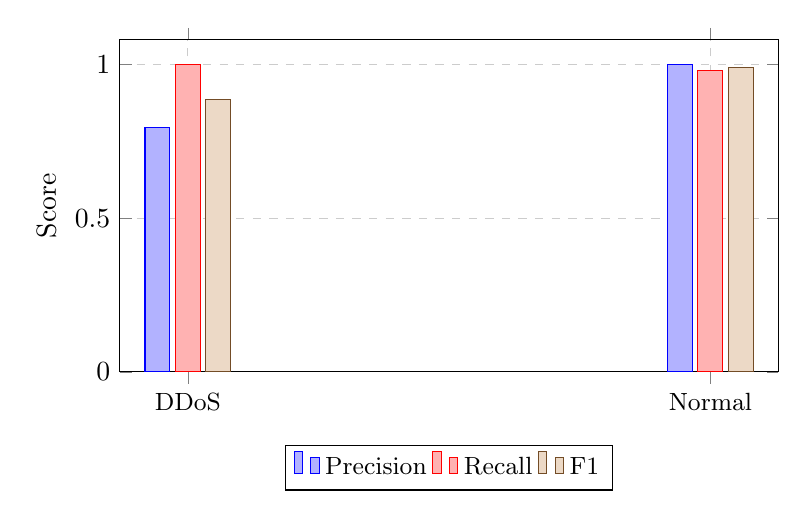
\begin{tikzpicture}
    \begin{axis}[
      ybar,
      bar width=9pt,
      ymin=0,
      ymax=1.08,
      ylabel={Score},
      symbolic x coords={DDoS, Normal},
      xtick=data,
      x tick label style={font=\small},
      legend style={font=\small, at={(0.5,-0.22)}, anchor=north, legend columns=3},
      width=0.82\textwidth,
      height=5.8cm,
      enlarge x limits=0.13,
      grid=major,
      major grid style={dashed, gray!40},
    ]
      \addplot coordinates {(DDoS,0.794) (Normal,1.000)};
      \addplot coordinates {(DDoS,1.000) (Normal,0.980)};
      \addplot coordinates {(DDoS,0.885) (Normal,0.990)};
      \legend{Precision,Recall,F1}
    \end{axis}
  \end{tikzpicture}
  \caption[Per-class P/R/F1 on test]{Per-class precision, recall, and F1 on the \textbf{test} split (Table~\ref{tab:perclass}).}
  \label{fig:prf}
\end{figure}

\subsection{\texorpdfstring{Blind test (0.3\,s test split)}{Blind test (0.3 s test split)}}
On the test split, class imbalance limits equal sampling: the maximum
equal-per-class blind size is 270 images (135 per class). With seed 42,
\path{scripts/blind_test_random.py} reports \textbf{98.9\%} accuracy and
macro F1 \textbf{0.989} (three normal images misclassified as DDoS).
Table~\ref{tab:blindcm} shows the blind-test confusion matrix.

\begin{table}[ht]
\centering
\caption[Blind test confusion matrix]{Blind test ($N=270$, seed 42, shuffled order). Rows\,=\,true class.}
\begin{tabular}{|c|c|c|}
\hline
 & \textbf{pred.\ DDoS} & \textbf{pred.\ normal} \\
\hline
true DDoS & 135 & 0 \\
\hline
true normal & 3 & 132 \\
\hline
\end{tabular}
\label{tab:blindcm}
\end{table}

\subsection{Legacy baseline: per-packet images}
An earlier per-packet pipeline on \texttt{dataset/images} achieved about
95.56\% test accuracy and a large 3000-image blind test with 99.9\% accuracy
(system description). That setup is distinct from the 0.3\,s window training
distribution. Table~\ref{tab:twopipes} contrasts the two experimental tracks.

\begin{table}[ht]
\centering
\small
\caption[Two experimental tracks]{Two experimental tracks in the repository (qualitative summary).}
\begin{tabular}{|>{\raggedright\arraybackslash}p{3.0cm}|>{\raggedright\arraybackslash}p{5.3cm}|>{\raggedright\arraybackslash}p{5.3cm}|}
\hline
 & \textbf{Per-packet images} & \textbf{0.3\,s window images (primary)} \\
\hline
Typical data path & \path{dataset/images} & \path{dataset/images_per_second_window_0p3} \\
\hline
Reported test acc. & ${\sim}$95.6\% & 98.10\% \\
\hline
Large blind test & 3000 images (${\sim}$99.9\% acc.) & max 270 balanced (98.9\%) \\
\hline
Loss / selection & Weighted CE / macro F1 (typ.) & Focal, early stop on val DDoS F1 \\
\hline
\end{tabular}
\label{tab:twopipes}
\end{table}

\subsection{Label-quality validation and cross-day generalization}
\label{sec:labelvalidation}
The primary results above rely on the SYN-count heuristic labeling
described in Section~\ref{sec:pipeline}\footnote{PCAP labeling and
packet-to-image encoding, Chapter~\ref{chapter:3}.}. To test whether that
heuristic limits generalization to attack traffic it did not shape, we
built a second, unsupervised labeling pipeline: $k$-means clustering on
per-window flow features (packet counts, SYN ratio, inter-arrival
statistics), accepting a cluster split as the attack label only if the
picked cluster's mean SYN ratio exceeds the other cluster's --- a
\emph{flood-signature gate} added specifically because the original
whole-day $k=2$ split could pass its silhouette gate while separating on
unrelated traffic volume rather than attack behavior (found on
\texttt{01-12-2018}, whose true SYN window is only about 5 minutes).
Where this gate fails, labeling falls back to the schedule-based labels
used elsewhere in this report. We paired the revised labels with a
\textbf{FlowPic}-style encoding~\cite{shapira2019flowpic}: each 0.3\,s
window becomes a $64\times64\times3$ packet-size$\times$arrival-time
histogram (all packets / SYN-only / ACK\,\textbar\,FIN\,\textbar\,RST
channels), log-scaled against a fixed global clip so absolute traffic
volume remains a real signal --- avoiding the natural-photo assumptions
(ImageNet augmentation and normalization statistics) that the byte-dump
encoding above carries despite being trained from scratch on packet
bytes, not photographs.

To stress-test generalization more strictly than the same-domain split
used for the primary model, we held out an \textbf{entire attack day}
(\texttt{01-12-2018}, 3 sub-pcap stems, 966 DDoS windows) as test and
trained only on the other attack day (\texttt{03-11-2018}, 8 stems, 1402
DDoS windows in train) plus normal-only captures split by whole source
PCAP (never by individual window, to avoid adjacent-window leakage across
splits). This is a genuine cross-day test: the model never sees any
window --- attack or normal --- from the held-out day's attack execution
during training.

The resulting model (\path{model/flowpic_0p3_validated_v1_continued/})
reached validation $\mathrm{f1\_ddos}=0.8656$ (epoch 16 of 18) but
held-out cross-day test $\mathrm{f1\_ddos}$ dropped to \textbf{0.419}
(Table~\ref{tab:gapfix}) --- a substantial same-checkpoint gap. Diagnosis
found 97\% of the 2{,}136 test false positives concentrated in exactly
the two sub-pcap stems containing the day's labeled DDoS windows, with a
1.68\% false-positive rate everywhere else in the held-out day (450
other stems, 5{,}370 normal windows). We cross-referenced the 2{,}071
flagged windows in those two stems against CICFlowMeter's official
per-flow \texttt{Label} column for \texttt{01-12-2018} --- independent of
both our derived labels and the model's own predictions --- and confirmed
\textbf{86 of 2{,}071} (4\%) are provably mislabeled by the
schedule-boundary heuristic (real attack traffic marked ``normal''
because the documented attack schedule window is narrower than the
actual attack). Relabeling only those 86 raises test $\mathrm{f1\_ddos}$
to \textbf{0.453}. The remaining 1{,}985 flagged windows fall outside the
official label file's narrow $\sim$4-minute coverage and cannot be
checked against it directly; feature statistics show them measurably
busier than confirmed true negatives in the same stem, but a visual
contact-sheet comparison shows they resemble sparse background traffic,
not the bright horizontal-line SYN-flood signature confirmed-DDoS images
show. We therefore report this as a real, only \emph{partially}
label-driven cross-day generalization gap, not as a pure labeling
artifact --- a more modest but more defensible claim than excluding the
two stems outright would have been.

\begin{table}[ht]
\centering
\caption[Cross-day test metrics, raw vs.\ corrected]{Cross-day test metrics on the validated-labels FlowPic model, before and after relabeling the 86 confirmed mislabels.}
\begin{tabular}{|l|c|c|}
\hline
\textbf{Metric} & \textbf{Raw} & \textbf{Corrected (86 relabeled)} \\
\hline
Accuracy & 0.7805 & 0.7889 \\
\hline
DDoS precision & 0.278 & 0.307 \\
\hline
DDoS recall & 0.851 & 0.863 \\
\hline
DDoS F1 & 0.419 & 0.453 \\
\hline
\end{tabular}
\label{tab:gapfix}
\end{table}

Two unsupervised baselines (a convolutional autoencoder and Deep
SVDD~\cite{ruff2018deep}, trained on normal-only windows with no DDoS
label ever seen) were also attempted on the same FlowPic representation,
as a check on whether anomaly detection could sidestep the labeling
question entirely. Both underperformed (test ROC AUC 0.60 and 0.52
respectively) for the same underlying reason: DDoS windows in this 0.3\,s
representation are sparser, not busier, than normal traffic, inverting
the usual ``anomaly = high reconstruction/distance error'' assumption
both methods rely on. We report this as a genuine negative result for
reconstruction- and distance-based unsupervised detection on this
representation, not a tuning failure.

\subsection{Deployment-oriented inference}
Live \path{run_pipeline.py} builds \textbf{per-packet} images within each
PCAP window; offline 0.3\,s training uses \textbf{window-aggregated} images.
The systemd unit uses \path{--window-sec 0.3} to align window duration with
training; monitor \path{detections.log} and tune \path{--max-images-per-window}
as needed. CPU inference uses the deployed checkpoint
\path{model/per_second_0p3_focal_v2/resnext50_32x4d_best.ckpt}
on the cloud host. Each log line records \texttt{pred} $\in \{\mathrm{ddos},
\mathrm{normal}\}$ and \path{p_ddos}; this is the classifier output, not
independent verification of an attack.

\subsection{Operational note: live traffic without labels}
On a public interface, many windows may receive \texttt{"pred": "ddos"} even when
no controlled attack was run: Internet background traffic (scans, bursts,
heterogeneous protocols) can differ from CICDDoS2019, and argmax labels treat
slight preference for the DDoS class as a full ``DDoS'' decision. High
\textbf{reported} attack rates in logs therefore indicate \textbf{model
suspicion}, not confirmed incidents. Operational use should consider a
confidence threshold on \texttt{p\_ddos}, consecutive-window rules, or hybrid
signals---left for future work.

\subsection{Limitations}
Same-domain offline scores do not guarantee the same error rate on the live
path (different image construction and traffic mix). Performance also depends on how closely
deployment traffic matches CICDDoS2019 labeling and windowing.
Per-window and imbalance-focused runs may differ from the default image-folder
training; adversarial traffic and payload encryption are out of scope for this
baseline. Section~\ref{sec:labelvalidation} investigates the SYN-count
labeling heuristic's effect on generalization directly: on a stricter
cross-day held-out test, a confirmed 4\% of false positives trace to the
labeling heuristic's schedule boundary, but the remaining gap reflects
genuine cross-day generalization difficulty, not primarily a labeling
artifact.


\chapter{Conclusion and Future Work}
\label{ch:conc}

This report presented an image-based SYN flood \gls{ddos} detector using
ResNeXt-50 and MindSpore, with the primary model trained on 0.3\,s time-window
images (\path{per_second_0p3_focal_v2}). On held-out test data from the
same distribution, accuracy was about 98.1\% with macro F1 about 0.94; blind
sampling confirmed strong performance within the limits of class balance.

To address the risk that the primary model's labels --- and consequently its
strong same-domain numbers --- merely reflect the SYN-count heuristic used to
generate them, Section~\ref{sec:labelvalidation} replaced that heuristic with
an unsupervised, cluster-validated labeling pipeline and re-evaluated under a
stricter cross-day held-out split (an entire attack day never seen in
training, not just unseen windows). That model reached
$\mathrm{f1\_ddos}=0.866$ on validation; cross-day test $\mathrm{f1\_ddos}$
was 0.419 raw, 0.453 after correcting 86 confirmed label-boundary mislabels
against the dataset's own official per-flow labels. We report this as a
real, partially-explained generalization gap rather than either dismissing
it as pure label noise or ignoring it --- the more defensible of the two
framings we considered this cycle. Two unsupervised anomaly-detection
baselines (autoencoder, Deep SVDD~\cite{ruff2018deep}) were also attempted on
the same revised labels and encoding; both underperformed for a specific,
diagnosed reason (DDoS windows are sparser, not busier, than normal traffic
in this 0.3\,s representation, inverting the anomaly-detection premise both
methods rely on) rather than from a tuning failure, which we record as a
genuine negative result.

Future work includes validation on additional datasets and attack types;
completing the byte-dump encoding under the same cluster-validated labels for
a full label-methodology $\times$ encoding ablation (in progress at the time
of writing); systematic comparison of time-window lengths and dual-view
(all-packets vs.\ SYN-only) fusion; hardware acceleration beyond CPU-only
deployment; stress-testing under concept drift, adversarial perturbations,
and \textbf{domain adaptation} when live packet-to-image rules differ from
offline windows; and \textbf{calibration} of live alerts (thresholds on
\path{p_ddos}, temporal smoothing, or hybrid rules) to reduce false positives
on real Internet traffic.


\chapter{Appendices}

\section{Threat model and scope}
The detector is trained on \textbf{CICDDoS2019-derived} images with labels from a
\textbf{SYN-centric heuristic} (PCAPs with many SYN flags treated as attack
traffic). It estimates whether a batch of packet images ``looks like'' the DDoS
class in that dataset. It does \textbf{not} by itself prove an ongoing
Internet-scale attack, identify the attacker, or cover non-TCP floods, UDP
floods, application-layer attacks, or encrypted traffic where byte patterns
differ from the training regime.

\section{Ethics and responsible use}
Capturing live traffic may include sensitive metadata. Logs should be
\textbf{access-controlled}; avoid publishing raw PCAPs from production.
\textbf{Misuse}: raising false alarms can disrupt operations; automated blocking
based solely on this model is discouraged without human review and tuning.
\textbf{Dual-use}: the same pipeline could be profiled for evasion; document
defensive intent and legal authorization for monitoring.

\section{Notation reference}
\begin{table}[ht]
\centering
\begin{tabular}{|l|l|}
\hline
\textbf{Symbol} & \textbf{Meaning} \\
\hline
$\mathcal{D}$ & Labeled image dataset \\
\hline
$y_i$ & Ground-truth class index (DDoS vs.\ normal) \\
\hline
$p_{\mathrm{ddos}}(\mathbf{x})$ & Softmax probability for DDoS class \\
\hline
$\tau$ & Threshold on $p_{\mathrm{ddos}}$ for operational alerts (optional) \\
\hline
\end{tabular}
\caption[Notation reference]{Notation used in Section~\ref{sec:notation} and the appendices.}
\label{tab:notationlist}
\end{table}

\section{Extended related work (selected)}
\begin{table}[ht]
\centering
\small
\begin{tabular}{|>{\raggedright\arraybackslash}p{2.6cm}|>{\raggedright\arraybackslash}p{3.0cm}|>{\raggedright\arraybackslash}p{3.0cm}|>{\raggedright\arraybackslash}p{3.6cm}|}
\hline
\textbf{Reference} & \textbf{Data / setting} & \textbf{Model family} & \textbf{Notes} \\
\hline
Bazzi et al.\ (BAU)~\cite{bazzi2022resnet} & CICDDoS2019, packet images & ResNet-50 & Baseline for packet-image SYN detection \\
\hline
Sharafaldin et al.~\cite{cic2019ddos} & CICDDoS2019 release & n/a (dataset) & Public DDoS benchmark \\
\hline
Xie et al.~\cite{xie2017aggregated} & ImageNet / vision & ResNeXt & Cardinality / grouped convolutions \\
\hline
Mirsky et al.~\cite{mirsky2019kitsune} & Network IDS context & Autoencoder kitsune & Deep traffic anomaly framing \\
\hline
Vinayakumar et al.~\cite{vinayakumar2019review} & Survey & CNN/RNN/ML & Broad DL-for-ID survey \\
\hline
\textbf{This work} & CICDDoS2019, 0.3\,s windows & ResNeXt-50, MindSpore & Huawei stack + live pipeline \\
\hline
\end{tabular}
\caption[Extended related-work positioning]{Positioning sketch (not an exhaustive literature review).}
\label{tab:extendedlit}
\end{table}

\section{Frequently asked questions}
\begin{description}
  \item[Why do live logs show many \texttt{ddos} lines without an attack?]
    The model performs \textbf{binary classification} on captured bytes; public
    Internet traffic and train/serve mismatch can yield false positives. See
    Section~\ref{ch:results} (operational note).
  \item[What do \texttt{alert} and \texttt{streak} mean in JSON logs?]
    \texttt{streak} counts consecutive windows where $p_{\mathrm{ddos}}$ meets
    \path{alert_min_p_ddos}; \texttt{alert} is true when the streak reaches
    \path{alert_consecutive}. Webhooks fire only when \texttt{alert} is true.
  \item[How do I reproduce the PDF figures?] Run
    \texttt{bash} \path{scripts/run_all_paper_figures.sh} (requires matplotlib and the
    evaluation dataset).
\end{description}

\section{Reproducibility checklist}
\begin{table}[ht]
\centering
\small
\begin{tabular}{|l|l|}
\hline
\textbf{Item} & \textbf{Snapshot (2026-04-03 GPU eval)} \\
\hline
Python & 3.10.12 \\
\hline
MindSpore & 2.6.0 \\
\hline
\texttt{mindcv} & 0.3.0 \\
\hline
Git commit & \path{96b82d4cf152053175950a346bdd204b6e109ebf} \\
\hline
\end{tabular}
\caption[Reproducibility environment]{Environment pinned for offline reproduction; see \path{reports/REPRODUCIBILITY.md} and \path{reports/pip_freeze_2026-04-03.txt}.}
\label{tab:reproenv}
\end{table}

\begin{itemize}
  \item \textbf{Code:} Huawei MindSpore + \path{mindcv}; Python 3 with project venv.
  \item \textbf{Checkpoint:} \path{model/per_second_0p3_focal_v2/resnext50_32x4d_best.ckpt}.
  \item \textbf{Data:} \path{dataset/images_per_second_window_0p3} (train/val/test).
  \item \textbf{Offline eval:} \texttt{bash} \path{scripts/run_all_eval_0p3.sh}.
  \item \textbf{Curves / ECE:} \path{scripts/eval_roc_pr_calibration.py} (defaults to \textbf{GPU}; \path{--device-target CPU} if needed).
  \item \textbf{Live:} \path{run_pipeline.py} \path{--live} with systemd unit in \path{depployemnt/systemd/}.
  \item \textbf{Log dashboard (static HTML):} \path{scripts/generate_log_dashboard.py} \path{--log} \path{/path/to/detections.log}.
\end{itemize}

\section{Optional analysis figures (generated)}
ROC, PR, threshold sweep, and confusion heatmaps are written as PDFs under
\path{research/figures/} when you run \path{scripts/eval_roc_pr_calibration.py}
or \path{scripts/run_all_paper_figures.sh}. On the 2026-04-03 GPU run,
\path{eval_roc_pr_calibration.py} reported approximate test ECE $\approx 0.074$
and a max-F1 heuristic threshold $\approx 0.87$ on softmax (see
\path{reports/paper_figures_2026-04-03.log}). Include figures in slides or theses
with \verb|\includegraphics| if present.

\IfFileExists{figures/roc_test.pdf}{%
\begin{figure}[ht]
  \centering
  
\includegraphics[width=0.55\textwidth]{figures/roc_test.pdf}
  \caption{ROC curve (test split), generated script output.}
  \label{fig:rocgen}
\end{figure}
}{}

\IfFileExists{figures/pr_test.pdf}{%
\begin{figure}[ht]
  \centering
  
\includegraphics[width=0.55\textwidth]{figures/pr_test.pdf}
  \caption{Precision--recall curve (test split), generated script output.}
  \label{fig:prgen}
\end{figure}
}{}

\IfFileExists{figures/confusion_heatmap_test.pdf}{%
\begin{figure}[ht]
  \centering
  
\includegraphics[width=0.42\textwidth]{figures/confusion_heatmap_test.pdf}
  \caption{Confusion matrix heatmap (test split).}
  \label{fig:cmheat}
\end{figure}
}{}

\section{Window-length experiments (repository scripts)}
Training scripts such as \path{train_resnext_per_second_0p3.sh},
\path{train_resnext_per_second_1s.sh}, and related folders under
\path{model/} support comparing 0.3\,s vs.\ 1\,s windows. A full sweep table is
\textbf{not} fixed here because metrics depend on the machine used; run the
corresponding \texttt{eval\_per\_second\_*.sh} scripts and paste results into
your defense slides.

\section{Feature-space visualization (future work)}
High-dimensional t-SNE or UMAP plots require exporting intermediate tensors from
MindSpore. See \path{scripts/extract_features_tsne.py} for the intended hook
point; not automated in this repository snapshot.


\renewcommand{\bibname}{References}
\cleardoublepage
\phantomsection
\addcontentsline{toc}{chapter}{References}
\bibliography{references}
\end{document}